
% !TEX encoding = UTF-8 Unicode 
% !TEX root = FieldGuide.tex

\Sec{Pearson VII Distribution}
\phantomsection\addcontentsline{toc}{subsection}{~~~~~~~~~~~~Pearson VII} 

The {\bf Pearson type VII} distribution~\cite{Pearson1916} is a three parameter, continuous, univariate, unimodal, symmetric probability distribution, with infinite support. The functional form in the most straight forward parameterization is
\begin{align}
\label{PearsonVII}
\opr{PearsonVII}(x\given a,s, m) 
%\\ \notag
&= \frac{1}{|s| B(m-\frac{1}{2}, \frac{1}{2} )} \left( 1 +\left( \frac{x-a}{s}\right)^2 \right)^{-m} 	\checked
\\ \notag
& \qquad m > \tfrac{1}{2}
\\ \notag & = \opr{PearsonIV}(x\given a,s, m,0)  \checked
\end{align}
This distribution family is notable for having long power-law tails in both directions. 


\SSec{Special cases}


\dist{Student's t} (Student, t, Student-Fisher, Fisher) distribution~\cite{Student1908,Fisher1925b,Hanley2008, Zabell2008} :
\begin{align}
\label{StudentsT}
\opr{StudentsT}(x\given k) 
&= \frac{1}{\sqrt{k} B(\frac{1}{2}, \frac{1}{2} k)} \left( 1 + \frac{x^2}{k} \right)^{-\frac{1}{2}(k+1)} \checked
\\ &= \opr{PearsonVII}(x\given 0,\sqrt{k},\tfrac{1}{2}(k+1)) \checked
\notag
\\ & \qquad \text{integer } k \geq 0
\notag
\end{align}
The distribution of the statistic $t$, which arises when considering the error of samples means drawn from normal random variables.
\begin{align*}
	t =& \sqrt{n} \frac {\bar{x} - \mu}{\bar{s}}  \checked \\ 
	\bar{x} & = \tfrac{1}{n} \sum_{i=1}^{n} \opr{Normal}_i (\mu,\sigma)   \checked \\
	\bar{s}^2 &= \tfrac{1}{n-1} \sum_{i=1}^{n} \bigl( \opr{Normal}_i (\mu,\sigma) - \bar{x} \bigr)^2 \checked
\end{align*}
Here, $\bar{x}$ is the sample mean of $n$ independent normal \eqref{Normal} random variables with mean $\mu$ and variance  $\sigma^2$, $\bar{s}$ is the sample variance, and $k=n-1$ is the `degrees of freedom'.


\begin{figure}[t]
\begin{center}
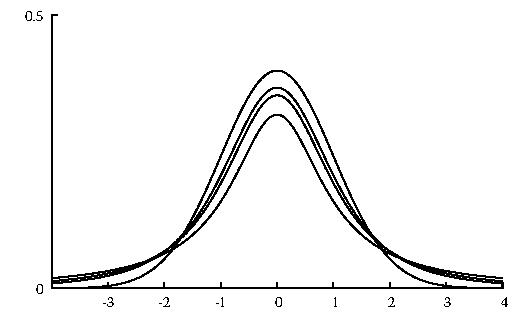
\includegraphics[width=\textwidth]{pdfStudentsT}
\end{center}
\caption[Student's t distributions]{Student's t distributions \eqref{StudentsT}: Cauchy ($k=1$), $t_2$ ($k=2$), $t_3$ ($k=3$), normal ($k\rightarrow\infty$) (low to high peak).}
\end{figure}

\begin{table*}[tp]
%\addcontentsline{toc}{subsection}{Cauchy} 
\begin{center}
\caption[Pearson VII distribution -- Special cases]{Special cases of the Pearson type VII distribution}
%\begin{align*}
%&\opr{PearsonIV}(x\given a,s, m,v) 
%\\ \notag &= \frac{{}_{2}F_1(-i\frac{v}{2}, i\frac{v}{2}, m;1)  }{s B(m-\frac{1}{2}, \frac{1}{2} )} \left( 1 +\left( \frac{x-a}{s}\right)^2 \right)^{-m}
% \exp \left\{ - 2v \arctan \left( \frac{x-a}{s}\right) \right\}
%\end{align*}
~\\
{\renewcommand{\arraystretch}{1.25}
\begin{tabular}{llcccl}
%\eqref{PearsonIV}&Pearson type IV & a & $s$ & $m$ &~$v$~ & 
\eqref{PearsonVII}&Pearson type VII & $a$ & $s$ & $m$  &  \\
 \hline
\eqref{StudentsT}& Student's $t$		& 0	& $\sqrt{k}$ & $\tfrac{k+1}{2}$  \\
\eqref{StudentsT2}& Student's $t_2$		& 0	& $\sqrt{2}$ & $\tfrac{3}{2}$  \\
\eqref{StudentsT3}& Student's $t_3$		& 0	& $\sqrt{3}$ & $2$  \\
\eqref{StudentsZ}& Student's $z$             	& 0 & 1&  n/2  \\
\eqref{Cauchy} &Cauchy 			& . & . & 1  \\
\eqref{StdCauchy} &standard Cauchy 			& 0 & 1 & 1  \\
\eqref{RelBreitWigner}& relativistic Breit-Wigner  & . & . & 2 \\
%\\
%& \underline{Limits} \\
%\eqref{Normal}& normal			& $\mu$ & $2\sigma^2 m^{\frac{1}{2}}$ & $m$ &$\lim_{m\rightarrow\infty}$ \\
\end{tabular} }
\end{center}
\end{table*}




\dist{Student's \texorpdfstring{$t_2$}{t2}} ($t_2$) distribution~\cite{Jones2002} :
\begin{align}
\label{StudentsT2}
\StudentsTT(x) 
&= \frac{1}{\left( 2 + x^2 \right)^{\frac{3}{2} } } \checked
\\ \notag 
& = \opr{StudentsT}(x\given 2) \checked
\\ \notag
&= \opr{PearsonVII}(x\given 0,\sqrt{2},\tfrac{3}{2}) \checked
\end{align}
Student's t distribution with 2 degrees of freedom has a particularly simple form. 

\dist{Student's \texorpdfstring{$t_3$}{t3}} ($t_3$) distribution~\cite{Devroye1986} :
\begin{align}
\label{StudentsT3}
\StudentsTTT(x)
&= \frac{2}{\pi \left( 1 + \tfrac{x^2}{3} \right)^{2} } \checked
\\ \notag 
& = \opr{StudentsT}(x\given 3) \checked
\\ \notag
& = \opr{RelBreitWigner}(x\given 0, \sqrt{3}, s) 
\\ \notag 
&= \opr{PearsonVII}(x\given 0,\sqrt{3},2) \checked
\end{align}
Student's t distribution with 3 degrees of freedom. Notable since the cumulative distribution function has a relatively simple form~\cite[p37]{Devroye1986}.
\[
\notag 
\op{StudentsT_3 CDF} (x) = \half + \sfrac{1}{\sqrt{3}\pi} \bigr( \arctan( \sfrac{x}{\sqrt{3}}) + \sfrac{\sfrac{x}{\sqrt{3}}}{1+\sfrac{x^2}{3}} \bigl) \checked
\]



\dist{Student's z}  distribution~\cite{Student1908,Hanley2008}:
\begin{align}
\label{StudentsZ}
\opr{StudentsZ}(z\given n) &= \frac{1}{B(\tfrac{n-1}{2}, \tfrac{1}{2})}  \left( 1 + z^2 \right)^{-\frac{n}{2} } \checked \\
&= \opr{PearsonVII}(z\given 0,1,\tfrac{n}{2}) \notag \checked
\end{align}
The distribution of the statistic $z$, which was the original distribution investigated by Gosset (aka Student)\footnote{Gosset's employer, the Guinness Brewing Company, insisted that he publish under a pseudonym.} in his famous 1908 paper
 on the statistical error of sample means~\cite{Student1908}.
\begin{align*}
	z &= \frac {\bar{x} - \mu}{s} \\ 
	\bar{x} &= \tfrac{1}{n} \sum_{i=1}^{n} \opr{Normal}_i (\mu,\sigma) \ , \\
	s^2 &= \tfrac{1}{n} \sum_{i=1}^{n} \bigl( \opr{Normal}_i (\mu,\sigma) - \bar{x} \bigr)^2
\end{align*}
Here, $\bar{x}$ is the sample mean of $n$ independent normal \eqref{Normal} random variables with mean $\mu$ and variance  $\sigma^2$, and $s^2$ is the sample variance, except normalized by $n$ rather than the now conventional $n-1$. Latter work by Student and Fisher~\cite{Fisher1925b} resulted in a switch to the statistic $t= z/\sqrt{n-1}$.


\dist{Cauchy} (Lorentz, Lorentzian, Cauchy-Lorentz,  Breit-Wigner, normal ratio, Witch of Agnesi) distribution~\cite{Poisson1827,Cauchy1853,Johnson1995}: 
% History see: Earliest Known Uses of Some of the Words of Mathematics
%
\begin{align}
\label{Cauchy}
\opr{Cauchy}(x\given a,s) &= \frac{1}{s \pi} \left( 1 +\left( \frac{x-a}{s}\right)^2 \right)^{-1}		\checked
\\  
&= \opr{PearsonVII}(x\given a,s,1)												\checked
\notag 
\end{align}

The Cauchy distribution is stable \eqref{Stable}\index{stable distributions}: a sum of independent Cauchy random variables is also Cauchy distributed.
\[
\opr{Cauchy}_1(a_1,s_1)  + \opr{Cauchy}_2(a_2,s_2) \sim \opr{Cauchy}_3(a_1+a_2,s_1+s_2) \checked
\notag
\]



\begin{figure}[t]
\begin{center}
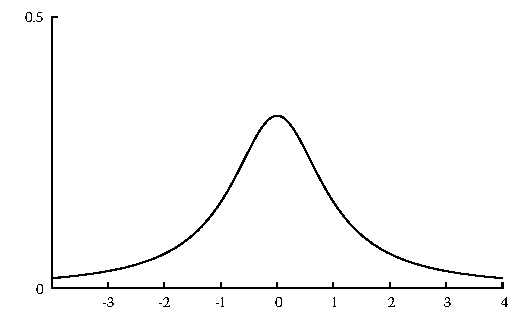
\includegraphics[width=\textwidth]{pdfCauchy}
\end{center}
\caption[Standard Cauchy distribution]{Standard Cauchy distribution, $\opr{StdCauchy}(x)$.}
\end{figure}



\dist{Standard Cauchy} distribution~\cite{Johnson1995}:
\begin{align}
\label{StdCauchy}
\opr{StdCauchy}(x) & = \frac{1}{\pi} \frac{1}{1+ x^2}				\checked
\\ 
\notag
& = \frac{1}{\pi} (x+i)^{-1} (x-i)^{-1} 							\checked
\\ \notag &= \opr{Cauchy}(x\given 0,1)						\checked
\\ \notag &= \opr{PearsonVII}(x\given 0,1,1)					\checked
\end{align}



\dist{Relativistic Breit-Wigner} (modified Lorentzian) distribution~\cite{Breit1936}:
\begin{align}
\label{RelBreitWigner}
\opr{RelBreitWigner}(x\given a, s) &= \frac{2}{ |s| \pi} \left( 1 +\left( \frac{x-a}{s}\right)^2 \right)^{-2} \checked
\\ \notag &= \opr{PearsonVII}(x\given a,s,2) \checked
\end{align}
Used to model the energy distribution of unstable particles in high-energy physics.



\SSec{Interrelations}

The Pearson VII distribution is a special case of the Pearson IV distribution~\eqref{PearsonIV}.
At high shape parameter $m$ the Pearson VII limits to the normal distribution.
\[
\opr{Normal}(x\given \mu,\sigma)   & = 
\lim_{m\rightarrow\infty} \opr{PearsonVII} ( x\given \mu, \sigma\sqrt{2m},m)
\notag
\checked
\]



The Pearson type VII distribution is given by a ratio of normal and gamma random variables
\cite[p445]{Devroye1986}.
\[
 \opr{PearsonVII}(a,s, m) \sim a+ s\sqrt{2m-1} \frac{\oprr{StdNormal}{Normal}()}{\sqrt{\opr{StdGamma}(m-\sfrac{1}{2})}} 
 \notag \checked
\]

The Cauchy distribution can be generated as a ratio of normal distributions
\[
 \opr{Cauchy}(0, 1) \sim \frac{\opr{Normal}_1(0,1)}{\opr{Normal}_2(0,1)}   \checked \notag
\]
and as a ratio of gamma distributions~\cite[p427]{Devroye1986}. %p427
\[
\Bigl(\opr{Cauchy}(0, 1)\Bigr)^2\sim  \frac{\opr{StdGamma}_1(\tfrac{1}{2})}{\opr{StdGamma}_2(\tfrac{1}{2})} 
\notag
\checked
\]




% !TEX encoding = UTF-8 Unicode 
% !TEX root = FieldGuide.tex

\begin{table*}[p]
\caption[Pearson VII distribution -- Properties]{Properties of the Pearson VII distribution}
\begin{align*}
\text{\hyperref[PropertiesSec]{Properties}}  \quad& \\
\text{notation} \quad & \text{PearsonVII}(x\given a,s, m) \checked
\\
\text{PDF}\quad &   \frac{1}{|s| B(m-\frac{1}{2}, \frac{1}{2} )} \Left( 1 +\Left( \frac{x-a}{s}\Right)^2 \Right)^{-m} \checked
\\
\text{CDF / CCDF} \quad  &  
     \frac{1}{2} +  \Left(\frac{x-a}{s}\Right) 
     \frac{1}{B(m-\frac{1}{2}, \frac{1}{2})}
     \,_2F_1 \Left ( \frac{1}{2},m;\frac{3}{2}; -\Left(\frac{x-a}{s}\Right)^2 \Right)
     \checked
     % Checked with Wolfram Alpha
     % D[1/2+ (x/s) Hypergeometric2F1[1/2, m , 3/2, -(x/s)^2] / Beta(m-1/2, 1/2), x]
     \hspace{-4em}
     \\
     &
\\
\text{parameters}\quad &   a,\ s,\ m  \in \Real \\ & m>\tfrac{1}{2} \checked
\\
\text{support} \quad &   -\infty < x < +\infty	\checked
\\
\text{median} \quad  &  a					\checked
\\
\text{mode} \quad  & a	\checked
\\
\text{mean} \quad  &  a & m>1	\checked
\\
\text{variance} \quad  & \frac{s^2}{2m-3} & m>\tfrac{3}{2} \checked
\\
\text{skew} \quad  &  0 \checked & m>2 \checked
\\
%\text{kurtosis} \quad  &  \cdots & m>\tfrac{5}{2}  
%\\ 
%\text{entropy} \quad  & \cdots
%\\
\text{MGF} \quad  &  \text{undefined}
\\
\text{CF} \quad  &   e^{iat} \frac{2 K_{m-\half} \Left( s |t|\Right)
                    \cdot \Left(\half s |t| \Right)^{m-\half}}
                    {\Gamma(m-\half)}  & m > \half
                    \checked
\end{align*}
\end{table*}

